\documentclass[a4,10pt]{aleph-notas}

\usepackage{booktabs}
\usepackage{array}
\usepackage{aleph-comandos}

\institucion{武汉大学}
\carrera{机器人工程}
\asignatura{人工智能与机器学习A}
\tema{章节课后作业}
\autor{Lai Wei}
\fecha{\today}
\logouno[5cm]{Logos/whulogo.png}

\newcommand{\qtitle}[1]{\subsection*{#1}\addcontentsline{toc}{subsection}{#1}}
\providecommand{\R}{\mathbb{R}}
\providecommand{\E}{\mathrm{E}}
\providecommand{\Var}{\mathrm{Var}}

\begin{document}

\encabezado
\tableofcontents

\section{第 1 章：概论}

\qtitle{一、名词解释}

\begin{ejer}[名词解释]
解释以下概念：特征空间、假设空间、标记空间。
\end{ejer}

\begin{description}[leftmargin=6em,style=nextline]
    \item[特征空间]
    样本用特征向量表示后可能取值的空间。若样本有 $d$ 个数值特征，常写为
    $\mathcal X\subseteq \R^d$，每个样本 $x=(x_1,\ldots,x_d)^T$ 是特征空间中的一个点。

    \item[假设空间]
    学习算法可能输出的模型或函数集合，记为 $\mathcal H$。学习过程本质上是在
    $\mathcal H$ 中根据训练数据选择一个假设 $h:\mathcal X\to\mathcal Y$。

    \item[标记空间]
    监督学习中样本标记可能取值的集合，记为 $\mathcal Y$。分类任务的标记空间通常是有限类别集合，
    回归任务的标记空间通常是实数集或实数向量空间。
\end{description}

\qtitle{二、回归与欠拟合/过拟合}

\begin{ejer}[回归与欠拟合/过拟合]
如下图是通过 GDP 对幸福度进行回归，蓝色点为已知样本，蓝色线表示回归曲线。
判断模型属于欠拟合还是过拟合，并解释欠拟合、过拟合的定义、对未知样本预测的影响及解决方法。
\begin{center}
    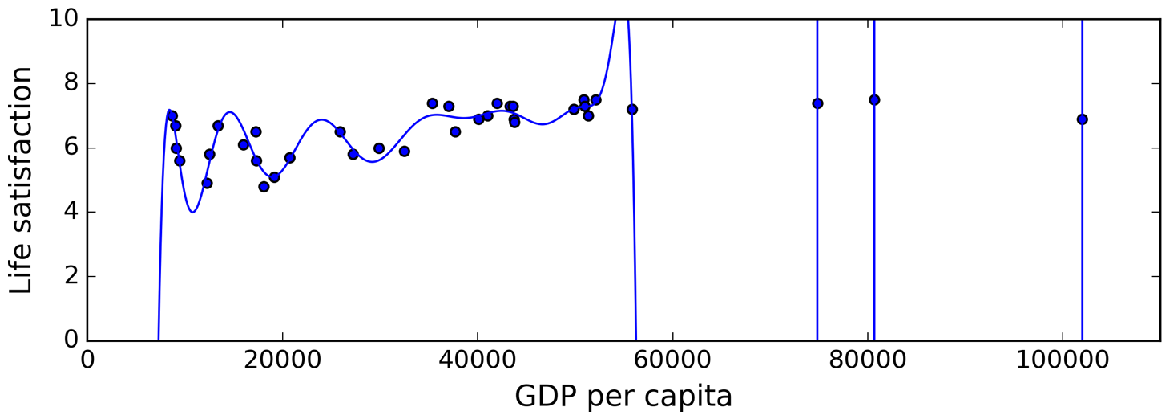
\includegraphics[width=0.78\linewidth]{ai_ml_practice/images/ch01_q02_gdp_regression.png}
\end{center}
\end{ejer}

\begin{enumerate}[label=（\arabic*）]
    \item 图中的蓝色回归曲线剧烈振荡，在训练样本附近刻意贴合，而在样本外区域出现不合理的垂直跳变，
    因此属于\textbf{过拟合}。

    \item 欠拟合指模型复杂度不足，连训练数据中的主要规律也没有学到，表现为训练误差和测试误差都较大。
    过拟合指模型把训练集中的噪声或偶然性也当成规律学习，表现为训练误差很小但泛化误差较大。
    欠拟合时，对未知样本的预测通常偏差较大；过拟合时，对未知样本的预测方差较大，对训练集以外的数据不稳定。

    \item 解决过拟合的常见方法包括降低模型复杂度、增加正则化、剪枝、早停、数据增强、扩大训练集、
    使用交叉验证选择超参数等。解决欠拟合的常见方法包括提高模型复杂度、加入更有效的特征、减弱正则化、
    延长训练或选择表达能力更强的模型。
\end{enumerate}

\qtitle{五、KNN 分类模型}

\begin{ejer}[KNN 分类模型]
KNN 分类模型中，$K$ 是什么意思？简述该模型的工作流程。
\end{ejer}

KNN 中的 $K$ 表示参与投票的最近邻样本个数。给定测试样本 $x$，KNN 的基本流程是：
计算 $x$ 与训练集中各样本的距离；选出距离最近的 $K$ 个样本；分类任务中按多数表决决定类别，
回归任务中通常取邻居标记的平均值或加权平均值。$K$ 较小时模型更敏感、方差较大；$K$ 较大时模型更平滑、偏差较大。

\section{第 2 章：模型选择与评估}

\qtitle{一、名词解释}

\begin{ejer}[名词解释]
解释以下概念：经验误差、泛化误差、训练集、测试集、验证集、查准率、查全率、分层采样、交叉验证、自助采样。
\end{ejer}

\begin{description}[leftmargin=6em,style=nextline]
    \item[经验误差] 学习器在训练集上的平均损失，也称训练误差。
    \item[泛化误差] 学习器在未知样本总体上的期望损失，反映模型对新数据的预测能力。
    \item[训练集] 用于拟合模型参数的数据集。
    \item[测试集] 训练完成后用于估计泛化性能的数据集，原则上不参与模型选择。
    \item[验证集] 训练过程中用于选择超参数、模型结构或早停轮数的数据集。
    \item[查准率] 预测为正的样本中真正为正的比例，
    $P=\dfrac{TP}{TP+FP}$。
    \item[查全率] 全部真实正例中被正确检出的比例，
    $R=\dfrac{TP}{TP+FN}$。
    \item[分层采样] 按类别比例分别抽样，使训练集、验证集、测试集尽量保持原始类别分布。
    \item[交叉验证] 将数据划分为若干份，轮流用其中一份验证、其余训练，并汇总多次验证结果估计性能。
    \item[自助采样] 从含 $m$ 个样本的数据集中有放回地抽取 $m$ 次形成训练集，未被抽中的样本可作包外测试。
\end{description}

\qtitle{四、ROC 与 AUC}

\begin{ejer}[ROC 与 AUC]
已知 8 个测试样本中有 4 个正例、4 个反例，预测结果为
\[
(s_1,0.80,+),(s_2,0.70,+),(s_3,0.56,-),(s_4,0.50,+),
\]
\[
(s_5,0.50,-),(s_6,0.30,+),(s_7,0.20,-),(s_8,0.15,-).
\]
画出 ROC 曲线，并给出 AUC 的值。
\end{ejer}

\textbf{基本概念：}ROC 曲线以假正例率 $FPR=FP/m_-$ 为横轴、
真正例率 $TPR=TP/m_+$ 为纵轴，通过移动分类阈值绘制。
AUC 为 ROC 曲线下方的面积（梯形法或排序法），值越接近 $1$ 分类器性能越好，
$0.5$ 表示随机猜测。

本题正例数和反例数均为 $m_+=m_-=4$。

\textbf{步骤一：按预测分数从高到低排序。}
\begin{center}
\begin{tabular}{ccc}
\toprule
样本 & 分数 & 真实标记\\
\midrule
$s_1$ & $0.80$ & $+$\\
$s_2$ & $0.70$ & $+$\\
$s_3$ & $0.56$ & $-$\\
$s_4$ & $0.50$ & $+$\\
$s_5$ & $0.50$ & $-$\\
$s_6$ & $0.30$ & $+$\\
$s_7$ & $0.20$ & $-$\\
$s_8$ & $0.15$ & $-$\\
\bottomrule
\end{tabular}
\end{center}

\textbf{步骤二：阈值依次降低，逐个（同分时同时）将样本纳入正类预测。}
$s_4$ 与 $s_5$ 分数相同（均为 $0.50$），在同一阈值处同时加入。
设 $TP$、$FP$ 为当前判断为正类的正例数和反例数，
则 $TPR=TP/4$、$FPR=FP/4$。

\begin{center}
\begin{tabular}{cccc}
\toprule
阈值区间 & 新增判为正类 & $TP$ & $FP$\\
\midrule
$>0.80$ & 无 & $0$ & $0$\\
$(0.70,0.80]$ & $s_1(+)$ & $1$ & $0$\\
$(0.56,0.70]$ & $s_2(+)$ & $2$ & $0$\\
$(0.50,0.56]$ & $s_3(-)$ & $2$ & $1$\\
$(0.30,0.50]$ & $s_4(+),s_5(-)$ & $3$ & $2$\\
$(0.20,0.30]$ & $s_6(+)$ & $4$ & $2$\\
$(0.15,0.20]$ & $s_7(-)$ & $4$ & $3$\\
$\leq0.15$ & $s_8(-)$ & $4$ & $4$\\
\bottomrule
\end{tabular}
\end{center}

\textbf{步骤三：计算各阈值对应的 (FPR, TPR) 坐标，即 ROC 曲线上的点。}

\begin{center}
\begin{tabular}{ccc}
\toprule
$(FPR,TPR)$ & $FPR=FP/4$ & $TPR=TP/4$\\
\midrule
$(0,0)$ & $0$ & $0$\\[6pt]
$(0,\dfrac14)$ & $0$ & $1/4$\\[6pt]
$(0,\dfrac12)$ & $0$ & $2/4$\\[6pt]
$(\dfrac14,\dfrac12)$ & $1/4$ & $2/4$\\[6pt]
$(\dfrac12,\dfrac34)$ & $2/4$ & $3/4$\\[6pt]
$(\dfrac12,1)$ & $2/4$ & $4/4$\\[6pt]
$(\dfrac34,1)$ & $3/4$ & $4/4$\\[6pt]
$(1,1)$ & $4/4$ & $4/4$\\[6pt]
\bottomrule
\end{tabular}
\end{center}

ROC 曲线的几何含义：从 $(0,0)$ 出发，先沿纵轴垂直上升（纯正例区间无FP），
遇负例后水平右移且伴随垂直上升（混合区间），最终到达右上角 $(1,1)$。

\textbf{步骤四：用梯形法计算 AUC。}
排除垂直线段（FPR 不变的部分），只对 FPR 发生变化的四段水平/斜向线段求梯形面积：

\[
\begin{aligned}
AUC &= \frac{\frac14}{2}\left(\frac12+\frac12\right)
     +\frac{\frac14}{2}\left(\frac12+\frac34\right) +\frac{\frac14}{2}\left(1+1\right)
     +\frac{\frac14}{2}\left(1+1\right) \\
    &= \frac18+\frac{5}{32}+\frac14+\frac14 \\
    &= \frac{25}{32} \approx 0.7813.
\end{aligned}
\]

\begin{figure}[H]
    \centering
    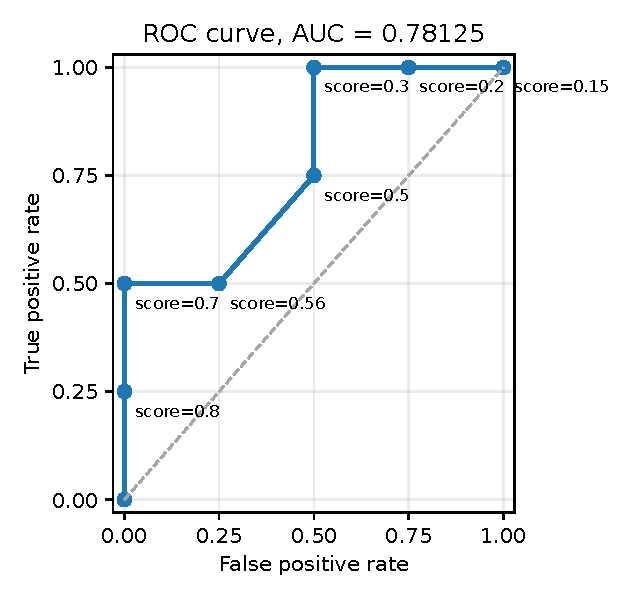
\includegraphics[width=0.52\linewidth]{solution_assets/ch02_roc.pdf}
    \caption{8 个测试样本的 ROC 曲线}
\end{figure}

\section{第 3 章：贝叶斯分类器}

\qtitle{一、名词解释}

\begin{ejer}[一、名词解释]
解释以下概念：后验概率、朴素贝叶斯分类器。
\end{ejer}

\begin{description}[leftmargin=6em,style=nextline]
    \item[后验概率]
    在观测到样本 $x$ 后，样本属于类别 $\omega_i$ 的条件概率
    $P(\omega_i\mid x)$。由贝叶斯公式，
    \[
        P(\omega_i\mid x)=
        \frac{P(x\mid\omega_i)P(\omega_i)}
        {\sum_j P(x\mid\omega_j)P(\omega_j)}.
    \]

    \item[朴素贝叶斯分类器]
    在给定类别条件下假设各特征条件独立的贝叶斯分类器。其判别规则为
    \[
        \hat y=\arg\max_{c} P(c)\prod_{j=1}^d P(x_j\mid c).
    \]
\end{description}

\qtitle{五、贝叶斯决策}

\begin{ejer}[五、贝叶斯决策]
假定对某一类人群进行疾病筛查，正常人群为 $\omega_1$，患者为 $\omega_2$，
设正常和患者的先验概率为：
\[
P(\omega_1)=0.7,\quad P(\omega_2)=0.3.
\]
现有一位被检查者，其观测值为 $x$，从类条件概率密度曲线上查得：
\[
P(x\mid \omega_1)=0.15,\quad P(x\mid \omega_2)=0.45.
\]
同时已知风险损失函数为：
\[
\begin{pmatrix}
\lambda_{11} & \lambda_{12}\\
\lambda_{21} & \lambda_{22}
\end{pmatrix}
=
\begin{pmatrix}
0 & 5\\
1 & 0
\end{pmatrix}.
\]
试对该被检查者用以下两种方式进行分类：
（1）用最小错误率的贝叶斯决策，并写出判别函数和决策方程；
（2）用最小风险的贝叶斯决策，并写出判别函数和决策方程。
\end{ejer}

先计算后验概率。未归一化后验为
\[
    P(x\mid\omega_1)P(\omega_1)=0.15\times0.7=0.105,
    \qquad
    P(x\mid\omega_2)P(\omega_2)=0.45\times0.3=0.135.
\]
归一化因子为 $P(x|\omega_1)P(\omega_1)+P(x|\omega_2)P(\omega_2)=0.24$，因此
\[
    P(\omega_1\mid x)=0.4375,\qquad
    P(\omega_2\mid x)=0.5625.
\]

\begin{enumerate}[label=（\arabic*）]
    \item 最小错误率贝叶斯决策的判别函数可取
    \[
        g_i(x)=P(x\mid\omega_i)P(\omega_i)
        \quad \text{或} \quad
        g_i(x)=P(\omega_i\mid x).
    \]
    决策方程为
    \[
        \hat\omega=\arg\max_i g_i(x).
    \]
    本题中
    \[
        g_1(x)=0.105,\qquad g_2(x)=0.135,
    \]
    因为 $g_2(x)>g_1(x)$，所以按最小错误率判为 $\omega_2$，即患者。

    \item 按贝叶斯决策中常用记号，设
    $\lambda_{ij}=\lambda(\alpha_i\mid\omega_j)$，即行对应采取的决策，
    列对应真实类别。风险判别函数可取
    \[
        r_i(x)=R(\alpha_i\mid x)=\sum_j \lambda_{ij}P(\omega_j\mid x),
    \]
    并选择风险较小的决策。
    损失矩阵是：
    \[
    \begin{pmatrix}
    \lambda_{11} & \lambda_{12}\\
    \lambda_{21} & \lambda_{22}
    \end{pmatrix}=
    \begin{pmatrix}
    0 & 5\\
    1 & 0
    \end{pmatrix}
    \]
    通常理解为：\(\lambda_{ij}\) 表示“把样本判为 \(\omega_i\)，但真实类别是 \(\omega_j\)”的损失。
    两个决策风险为
    \[
        R(\alpha_1\mid x)=0\cdot P(\omega_1\mid x)+5P(\omega_2\mid x)=2.8125,
    \]
    \[
        R(\alpha_2\mid x)=1\cdot P(\omega_1\mid x)+0\cdot P(\omega_2\mid x)=0.4375.
    \]
    最小风险决策方程为
    \[
        \hat\alpha=\arg\min_i R(\alpha_i\mid x).
    \]
    因为 $R(\alpha_2\mid x)<R(\alpha_1\mid x)$，所以按最小风险判为 $\omega_2$，即患者。
    等价地，当
    \[
        5P(\omega_2\mid x)<P(\omega_1\mid x)
    \]
    时判为正常，否则判为患者；本题不满足该不等式。
\end{enumerate}

\qtitle{六、朴素贝叶斯分类器}

\begin{ejer}[六、朴素贝叶斯分类器]
请从下列样本中构造一个朴素贝叶斯分类器，确定样本 $x=(2020,\ P)^T$ 的类别。
样本 $x$ 具有二维特征属性，取值分别为 $\{2019,2020,2021\}$ 和 $\{P,N,T\}$，
$y$ 为监督标记 $\{-1,1\}$，代表正类和反类。

\begin{center}
\scriptsize
\resizebox{\linewidth}{!}{%
\begin{tabular}{c|ccccccccccccccc}
\toprule
$i$ & 1 & 2 & 3 & 4 & 5 & 6 & 7 & 8 & 9 & 10 & 11 & 12 & 13 & 14 & 15\\
\midrule
$x_1$ & 2019 & 2019 & 2019 & 2019 & 2019 & 2020 & 2020 & 2020 & 2020 & 2020 & 2021 & 2021 & 2021 & 2021 & 2021\\
$x_2$ & P & N & N & P & P & P & N & N & T & T & T & N & N & T & T\\
$y$ & -1 & -1 & 1 & 1 & -1 & -1 & -1 & 1 & 1 & 1 & 1 & 1 & 1 & 1 & -1\\
\bottomrule
\end{tabular}%
}
\end{center}
\end{ejer}

由样本表统计得
\[
    P(y=1)=\frac{9}{15}=\frac35,\qquad
    P(y=-1)=\frac{6}{15}=\frac25.
\]
题目未要求平滑，朴素贝叶斯分类器取
\[
    \hat y=\arg\max_{c\in\{-1,1\}}
    P(y=c)P(x_1=2020\mid y=c)P(x_2=P\mid y=c).
\]
各条件概率为
\[
    P(x_1=2020\mid y=1)=\frac{3}{9}=\frac13,\qquad
    P(x_2=P\mid y=1)=\frac{1}{9},
\]
\[
    P(x_1=2020\mid y=-1)=\frac{2}{6}=\frac13,\qquad
    P(x_2=P\mid y=-1)=\frac{3}{6}=\frac12.
\]
于是
\[
    P(y=1)\prod_jP(x_j\mid y=1)
    =\frac35\cdot\frac13\cdot\frac19
    =\frac1{45},
\]
\[
    P(y=-1)\prod_jP(x_j\mid y=-1)
    =\frac25\cdot\frac13\cdot\frac12
    =\frac1{15}.
\]
由于 $\dfrac1{15}>\dfrac1{45}$，故
\[
    \hat y=-1.
\]
因此样本 $x=(2020,P)^T$ 的预测类别为标签 $-1$ 所对应的类别。

\section{第 4 章：线性模型}

\qtitle{一、名词解释}

\begin{ejer}[名词解释]
解释以下概念：基函数、联系函数、支持向量（SV）、梯度下降法、交叉熵、代价函数。
\end{ejer}

\begin{description}[leftmargin=6em,style=nextline]
    \item[基函数] 将原始输入映射为新特征的函数，如 $\phi_j(x)$。线性模型可写为
    $f(x)=\sum_j w_j\phi_j(x)$。
    \item[联系函数] 广义线性模型中连接条件均值与线性预测项的函数，如逻辑回归中的 logit 函数。
    \item[支持向量] SVM 中位于间隔边界上或违反间隔约束、对分类超平面起决定作用的训练样本。
    \item[梯度下降法] 沿目标函数负梯度方向迭代更新参数的方法：
    $\theta\leftarrow\theta-\eta\nabla_\theta J(\theta)$。
    \item[交叉熵] 衡量真实分布 $p$ 与预测分布 $q$ 差异的损失，
    $H(p,q)=-\sum_i p_i\log q_i$。
    \item[代价函数] 学习算法需要最小化的总体目标函数，通常由经验损失和正则化项组成。
\end{description}

\qtitle{三、一对多判别边界}

\begin{ejer}[一对多判别边界]
假设三个 $\omega_1,\omega_2,\omega_3$ 判别函数为：
$$
\begin{cases}
g_1(x)=-x_1-x_2+5\\
g_2(x)=-x_1+3\\
g_3(x)=-x_1+x_2
\end{cases}
$$
请画图给出一对多情况下的判别边界，以及三个类别的判别区域，并判断样本 $(1,3)$ 及 $(4,5)$ 的类别，如果不能确定其类别，请说明原因。
\end{ejer}

三个边界分别为
\[
    g_1(x)=0:\ x_1+x_2=5,\qquad
    g_2(x)=0:\ x_1=3,\qquad
    g_3(x)=0:\ x_2=x_1.
\]
一对多分类中，若恰有一个判别函数为正，则判为对应类别；若多个为正或全为负，则类别不能唯一确定。
因此三个确定分类区域为
\[
\omega_1:\ g_1>0,\ g_2<0,\ g_3<0,
\]
\[
\omega_2:\ g_2>0,\ g_1<0,\ g_3<0,
\]
\[
\omega_3:\ g_3>0,\ g_1<0,\ g_2<0.
\]
对样本 $(1,3)$，
\[
    (g_1,g_2,g_3)=(1,2,2),
\]
三个分类器均给出正类，发生冲突，类别不能确定。对样本 $(4,5)$，
\[
    (g_1,g_2,g_3)=(-4,-1,1),
\]
仅 $g_3>0$，故判为 $\omega_3$。

\begin{figure}[H]
    \centering
    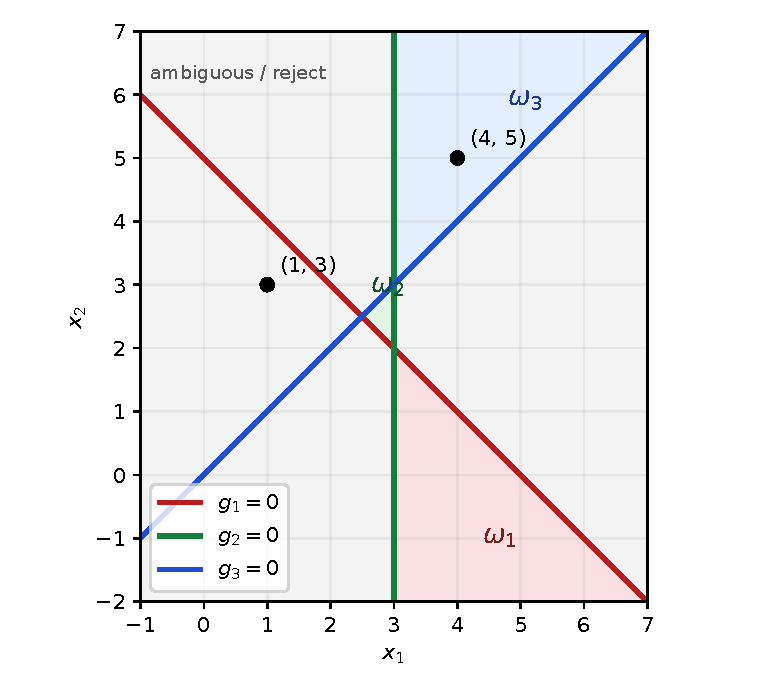
\includegraphics[width=0.62\linewidth]{solution_assets/ch04_ovr_regions.pdf}
    \caption{一对多判别边界与确定分类区域}
\end{figure}

\qtitle{四、LDA 投影}

\begin{ejer}[LDA 投影]
计算题：

（1）假设 LDA 最佳投影直线确定为 $5x_1-2x_2+1=0$。试求向量 $\begin{pmatrix}2\\0\end{pmatrix}$、$\begin{pmatrix}-1\\-7\end{pmatrix}$ 在该直线的 LDA 投影；

（2）推导样本在直线 $w$ 上投影点的协方差为 $w^T\Sigma_0 w$。
\end{ejer}

\begin{enumerate}[label=（\arabic*）]
    \item 直线为 $5x_1-2x_2+1=0$，法向量 $n=(5,-2)^T$。
    点 $x$ 到该直线的正交投影为
    \[
        x'=x-\frac{n^Tx+1}{\|n\|^2}n,\qquad \|n\|^2=29.
    \]
    对 $x=(2,0)^T$，
    \[
        x'=(2,0)^T-\frac{11}{29}(5,-2)^T
        =\left(\frac{3}{29},\frac{22}{29}\right)^T.
    \]
    对 $x=(-1,-7)^T$，
    \[
        x'=(-1,-7)^T-\frac{10}{29}(5,-2)^T
        =\left(-\frac{79}{29},-\frac{183}{29}\right)^T.
    \]

    \item 设样本 $x$ 的均值为 $\mu$，协方差为 $\Sigma_0=\E[(x-\mu)(x-\mu)^T]$。
    在方向 $w$ 上的一维投影为 $z=w^Tx$，则
    \[
        \Var(z)=\E[(w^Tx-w^T\mu)^2]
        =\E[w^T(x-\mu)(x-\mu)^Tw]
        =w^T\Sigma_0w.
    \]
\end{enumerate}

\qtitle{七、交叉熵损失}

\begin{ejer}[交叉熵损失]
已知 10 个二分类样本的分类标签依次为 $(0,1,1,1,0,0,0,0,1,0)$，其中 $1$ 为正类标签，$0$ 为负类标签。
分类器预测结果如下：

\begin{center}
\begin{tabular}{ccccccccccc}
\toprule
样本 & 1 & 2 & 3 & 4 & 5 & 6 & 7 & 8 & 9 & 10\\
\midrule
正类概率 & 0.1 & 0.88 & 0.92 & 0.65 & 0.2 & 0.3 & 0.4 & 0.1 & 0.85 & 0.1\\
负类概率 & 0.9 & 0.12 & 0.08 & 0.35 & 0.8 & 0.7 & 0.6 & 0.9 & 0.15 & 0.9\\
\bottomrule
\end{tabular}
\end{center}

请计算这 10 个样本的交叉熵损失。
\end{ejer}

交叉熵只需要取每个样本“真实类别对应的预测概率”。

二分类交叉熵取自然对数：
\[
    L=-\sum_{i=1}^{10}\left[
    y_i\log p_i+(1-y_i)\log(1-p_i)
    \right].
\]
10 个样本真实类别对应概率分别是：
\[
0.9,0.88,0.92,0.65,0.8,0.7,0.6,0.9,0.85,0.9
\]
逐项相加得
\[
\begin{aligned}
    L&=-(\ln0.9+\ln0.88+\ln0.92+\ln0.65+\ln0.8+\ln0.7+\ln0.6+\ln0.9+\ln0.85+\ln0.9) \\
    &=2.2112.
\end{aligned}
\]
若按样本平均，则
\[
    \bar L=\frac{L}{10}=0.2211.
\]

\section{第 5 章：决策树}

\qtitle{一、名词解释}

\begin{ejer}[名词解释]
解释以下概念：熵和条件熵、信息增益、基尼指数。
\end{ejer}

\begin{description}[leftmargin=6em,style=nextline]
    \item[熵和条件熵]
    熵衡量随机变量不确定性：
    $H(Y)=-\sum_k p_k\log_2p_k$。
    条件熵衡量给定 $X$ 后 $Y$ 的平均不确定性：
    $H(Y\mid X)=\sum_xP(X=x)H(Y\mid X=x)$。

    \item[信息增益]
    用属性 $A$ 划分数据集 $D$ 后不确定性的减少量：
    \[
        Gain(D,A)=H(D)-H(D\mid A).
    \]
    ID3 每次选择信息增益最大的属性。

    \item[基尼指数]
    CART 分类树常用的不纯度指标：
    \[
        Gini(D)=1-\sum_kp_k^2.
    \]
    基尼指数越小，节点越纯。
\end{description}

\qtitle{四、最小二乘回归树}

\begin{ejer}[最小二乘回归树]
根据样本
\[
x=(1,2,\ldots,10),\quad
y=(4.5,4.75,4.91,5.34,5.8,7.05,7.9,8.23,8.7,9.5),
\]
生成一个深度 \texttt{depth=3} 的最小二乘回归树并作图。
\end{ejer}

采用 CART 最小二乘准则，对每个候选切分点 $s$ 计算
\[
    \sum_{x_i\le s}(y_i-\bar y_L)^2+\sum_{x_i>s}(y_i-\bar y_R)^2.
\]
将根节点深度记为 $0$，取 \texttt{max\_depth=3}。根节点候选切分中，
$s=5.5$ 的误差最小，误差为 $4.3827$，因此先切分为
$x\le5.5$ 与 $x>5.5$。
继续递归切分得到
\[
\begin{aligned}
x\le5.5 &: \quad x\le3.5,\quad
    (x\le1.5),\ (x\le4.5),\\
x>5.5 &: \quad x\le8.5,\quad
    (x\le6.5),\ (x\le9.5).
\end{aligned}
\]
最终叶节点预测值为各叶节点内样本 $y$ 的均值：
\begin{center}
\begin{tabular}{cc}
\toprule
区间 & 预测值\\
\midrule
$x\le1.5$ & $4.50$\\
$1.5<x\le3.5$ & $4.83$\\
$3.5<x\le4.5$ & $5.34$\\
$4.5<x\le5.5$ & $5.80$\\
$5.5<x\le6.5$ & $7.05$\\
$6.5<x\le8.5$ & $8.065$\\
$8.5<x\le9.5$ & $8.70$\\
$x>9.5$ & $9.50$\\
\bottomrule
\end{tabular}
\end{center}

\begin{figure}[htbp]
    \centering
    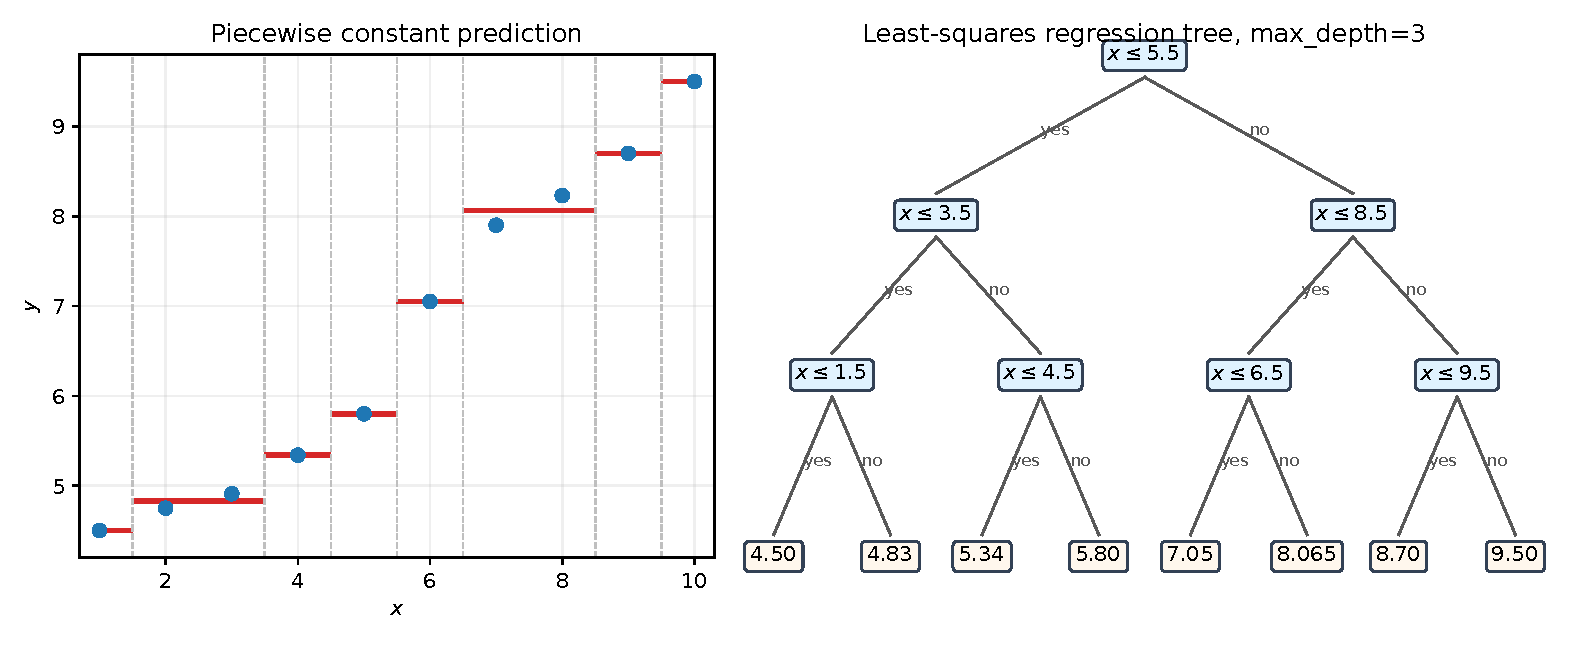
\includegraphics[width=0.5\linewidth]{solution_assets/ch05_regression_tree.pdf}
    \caption{深度为 3 的最小二乘回归树}
\end{figure}

\qtitle{五、ID3 与 CART 决策树}

\begin{ejer}[ID3 与 CART 决策树]
对题中给出的贷款申请样本表，分别用 ID3 和 CART 算法生成决策树，并写出主要计算步骤。
属性包括年龄、有工作、有自己的房子、信贷情况，类别为是否批准。
\end{ejer}

数据集中正例 ``是'' 有 $12$ 个，反例 ``否'' 有 $6$ 个，因此
\[
    H(D)=-\frac{12}{18}\log_2\frac{12}{18}
          -\frac{6}{18}\log_2\frac{6}{18}
        =0.9183.
\]
各属性的信息增益为
\begin{center}
\begin{tabular}{cc}
\toprule
属性 & $Gain(D,A)$\\
\midrule
年龄 & $0.0285$\\
有工作 & $0.3789$\\
有自己的房子 & $0.4591$\\
信贷情况 & $0.3572$\\
\bottomrule
\end{tabular}
\end{center}
最大者为 ``有自己的房子''，故 ID3 根节点选择该属性。
当 ``有自己的房子=是'' 时，9 个样本全部为 ``是''，直接为叶节点。
当 ``有自己的房子=否'' 时，子集含 6 个 ``否''、3 个 ``是''，熵仍为 $0.9183$。
在该子集上
\begin{center}
\begin{tabular}{cc}
\toprule
属性 & $Gain$\\
\midrule
年龄 & $0.2516$\\
有工作 & $0.9183$\\
信贷情况 & $0.4739$\\
\bottomrule
\end{tabular}
\end{center}
故继续按 ``有工作'' 划分；``有工作=否'' 的样本全为 ``否''，
``有工作=是'' 的样本全为 ``是''。ID3 决策树为
\[
\begin{array}{l}
\text{若有自己的房子=是，则类别=是；}\\
\text{若有自己的房子=否 且 有工作=是，则类别=是；}\\
\text{若有自己的房子=否 且 有工作=否，则类别=否。}
\end{array}
\]

CART 使用基尼指数。根节点
\[
    Gini(D)=1-\left(\frac{12}{18}\right)^2-\left(\frac{6}{18}\right)^2=0.4444.
\]
对多值离散属性取最优二分切分时，各属性最小加权基尼指数为
\begin{center}
\begin{tabular}{cc}
\toprule
属性 & 最小加权 $Gini$\\
\midrule
年龄 & $0.4308$\\
有工作 & $0.2667$\\
有自己的房子 & $0.2222$\\
信贷情况 & $0.2769$\\
\bottomrule
\end{tabular}
\end{center}
最小者仍为 ``有自己的房子''，切分为
``否'' 与 ``是''。``有自己的房子=是'' 分支纯度为 $0$。
在 ``有自己的房子=否'' 子集上，继续按 ``有工作'' 切分时加权基尼指数为 $0$，
两个分支均纯。因此 CART 树与上面的 ID3 树结构一致。

\section{第 6 章：集成学习}

\qtitle{一、名词解释}

\begin{ejer}[名词解释]
解释概念：基学习器。
\end{ejer}

\begin{description}[leftmargin=6em,style=nextline]
    \item[基学习器]
    集成学习中被组合的单个学习器，也称个体学习器或弱学习器。多个基学习器通过投票、加权投票、
    平均或堆叠等方式形成集成模型。
\end{description}

\qtitle{二、AdaBoost 权重迭代关系}

\begin{ejer}[AdaBoost 权重迭代关系]
复习 AdaBoost 算法，推导样本 $x_i$ 第 $t$ 轮权重与第 $t+1$ 轮权重满足
\[
w_{t+1,i}=\begin{cases}
\dfrac{w_{t,i}}{2(1-e_t)}, & \text{分类正确},\\[6pt]
\dfrac{w_{t,i}}{2e_t}, & \text{分类错误}.
\end{cases}
\]
\end{ejer}

AdaBoost 第 $t$ 轮样本权重更新为
\[
    w_{t+1,i}=\frac{w_{t,i}\exp(-\alpha_ty_ih_t(x_i))}{Z_t},
    \qquad
    \alpha_t=\frac12\ln\frac{1-e_t}{e_t}.
\]
其中 $y_ih_t(x_i)=1$ 表示分类正确，$y_ih_t(x_i)=-1$ 表示分类错误。
归一化因子为
\[
    Z_t=(1-e_t)e^{-\alpha_t}+e_te^{\alpha_t}
        =2\sqrt{e_t(1-e_t)}.
\]
若分类正确，
\[
    w_{t+1,i}=
    \frac{w_{t,i}e^{-\alpha_t}}{Z_t}
    =\frac{w_{t,i}}{2(1-e_t)}.
\]
若分类错误，
\[
    w_{t+1,i}=
    \frac{w_{t,i}e^{\alpha_t}}{Z_t}
    =\frac{w_{t,i}}{2e_t}.
\]
这正是题中给出的迭代关系。

\qtitle{三、AdaBoost 强分类过程}

\begin{ejer}[AdaBoost 强分类过程]
给定 10 个训练样本和弱学习器
\[
h_1=\begin{cases}1,&X_1<2.5\\-1,&X_1>2.5\end{cases},\quad
h_2=\begin{cases}1,&X_1<8.5\\-1,&X_1>8.5\end{cases},\quad
h_3=\begin{cases}1,&X_2>6.5\\-1,&X_2<6.5\end{cases}.
\]
用 AdaBoost 算法实现强分类过程。
\begin{center}
    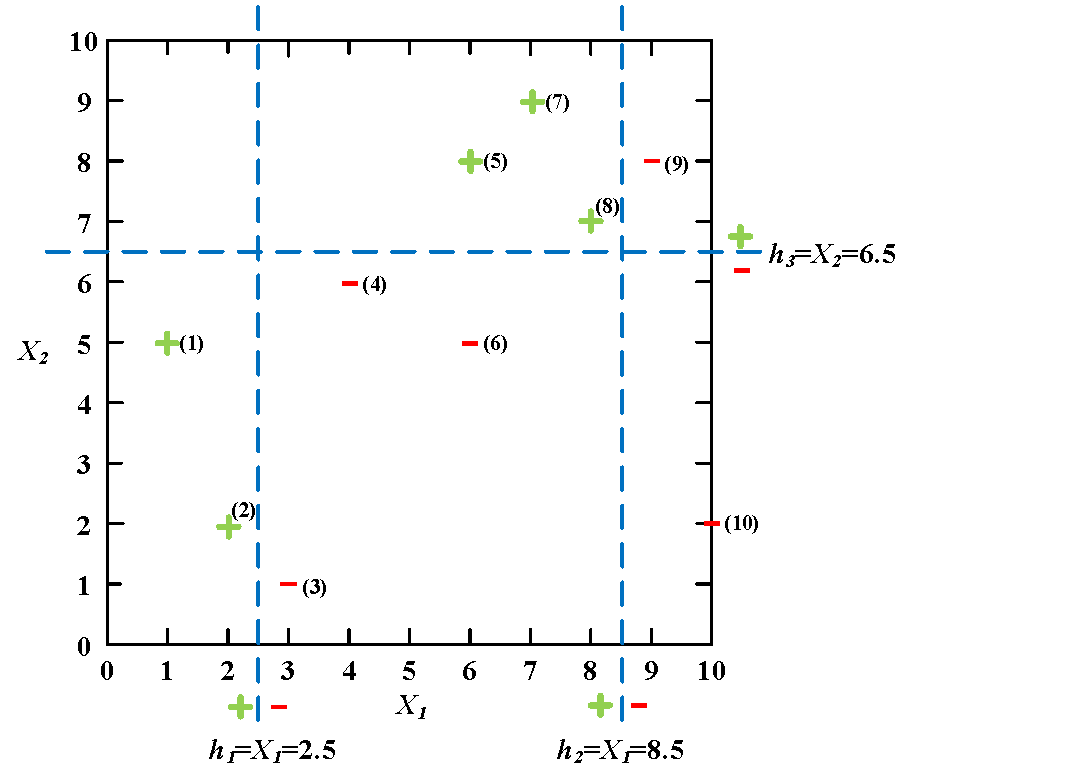
\includegraphics[width=0.55\linewidth]{ai_ml_practice/images/ch06_q03_adaboost_figure.png}
\end{center}
\end{ejer}

初始权重 $D_1(i)=0.1$。三个弱分类器第一轮错误率均为 $0.3$，
按题目给出的顺序选 $h_1$。计算过程为
\begin{center}
\begin{tabular}{ccccc}
\toprule
$t$ & $h_t$ & 错分样本 & $e_t$ & $\alpha_t$\\
\midrule
$1$ & $h_1$ & $5,7,8$ & $3/10$ & $\frac12\ln\frac73=0.4236$\\
$2$ & $h_2$ & $3,4,6$ & $3/14$ & $\frac12\ln\frac{11}{3}=0.6496$\\
$3$ & $h_3$ & $1,2,9$ & $3/22$ & $\frac12\ln\frac{19}{3}=0.9229$\\
\bottomrule
\end{tabular}
\end{center}
因此强分类器为
\[
    H(x)=\operatorname{sign}\left(
    0.4236h_1(x)+0.6496h_2(x)+0.9229h_3(x)
    \right).
\]
对 10 个训练样本，强分类器的加权输出符号为
\[
    (+,+,-,-,+,-,+,+,-,-),
\]
与给定类别完全一致。

\section{第 7 章：维度归约}

\qtitle{一、名词解释}

\begin{ejer}[名词解释]
解释概念：测地线（geodesic）距离。
\end{ejer}

\begin{description}[leftmargin=6em,style=nextline]
    \item[测地线距离]
    在流形或曲面上沿该流形可行路径连接两点的最短路径长度。与欧氏距离不同，测地线距离考虑数据所在流形的弯曲结构。
\end{description}

\qtitle{四、正交投影矩阵}

\begin{ejer}[正交投影矩阵]
降维分析中涉及投影的变换矩阵通常要求正交。说明正交投影矩阵相对于非正交投影矩阵的优点，
并解释为什么 PCA 中变换矩阵一定可以取为正交矩阵。
\end{ejer}

\begin{enumerate}[label=（\arabic*）]
    \item 正交投影矩阵的列向量相互正交且通常归一化，优点是投影后的坐标不冗余，
    不会人为引入斜交坐标造成的尺度耦合；长度、角度和方差解释更清楚，数值计算也更稳定。
    非正交投影可能把不同方向的信息混在一起，使投影坐标相关，解释性和重构分析都较差。

    \item PCA 的投影方向来自样本协方差矩阵的特征向量。协方差矩阵是实对称矩阵，
    不同特征值对应的特征向量正交；重特征值对应的特征子空间也可以选取一组正交规范基。
    因此 PCA 的变换矩阵可取为正交矩阵。
\end{enumerate}

\qtitle{五、PCA 与 LDA 投影方向}

\begin{ejer}[PCA 与 LDA 投影方向]
参照题图，绘制一个二维数据集示例，使 PCA 和 LDA 找到相同的好方向；
再绘制一个数据集，使 PCA 和 LDA 都找不到好的投影方向。
\begin{center}
    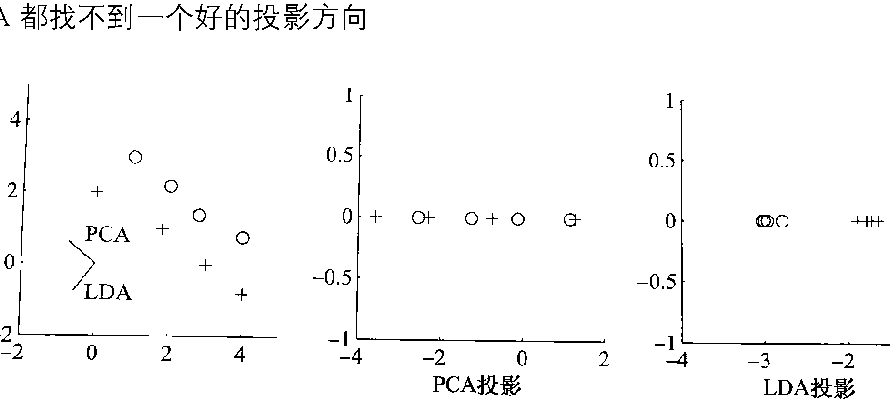
\includegraphics[width=0.55\linewidth]{ai_ml_practice/images/ch07_q05_pca_lda_figure.png}
\end{center}
\end{ejer}

当两类样本的均值差方向也是总方差最大的方向时，PCA 和 LDA 会找到相同的好方向。
例如两团数据左右分离，主要差异在 $x$ 轴方向。相反，XOR 型数据中两类均值相同，
类别信息不是任何单一线性投影能表达的；PCA 只看总体方差，LDA 的类均值差又为零，
两者都找不到好的投影方向。

\begin{figure}[H]
    \centering
    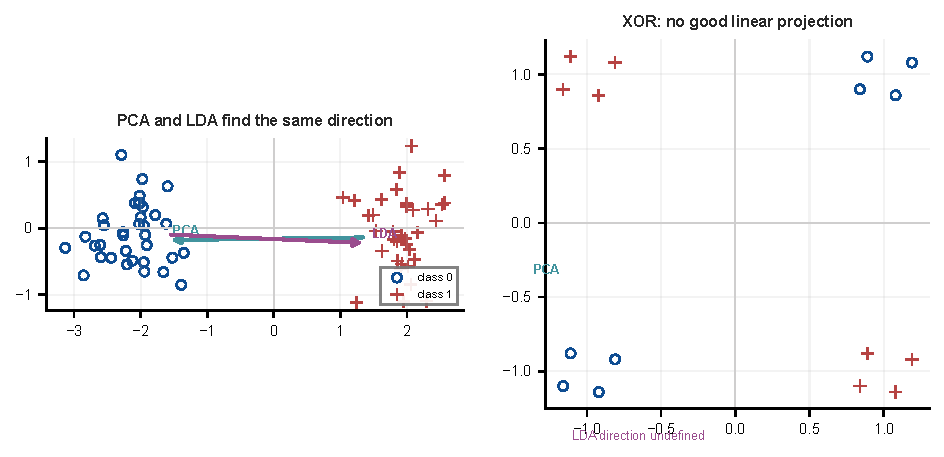
\includegraphics[width=0.92\linewidth]{solution_assets/ch07_pca_lda_examples.pdf}
    \caption{PCA 与 LDA 投影方向示例}
\end{figure}

\qtitle{六、PCA 主分量与方差贡献率}

\begin{ejer}[PCA 主分量与方差贡献率]
用 PCA 方法计算 6 个二维样本
\[
\begin{pmatrix}
2&3&3&4&5&7\\
2&4&5&5&6&8
\end{pmatrix}
\]
的一维 PCA 主分量，并计算该主分量的方差贡献率。注意：样本未中心化。
\end{ejer}

题目给出的样本未中心化，先求均值
\[
    \mu=\left(4,5\right)^T.
\]
中心化后的样本为
\[
X_c=
\begin{pmatrix}
-2&-1&-1&0&1&3\\
-3&-1&0&0&1&3
\end{pmatrix}.
\]
协方差矩阵可取
\[
    \Sigma=\frac1{6}X_cX_c^T
    =
    \begin{pmatrix}
    2.6667 & 2.8333\\
    2.8333 & 3.3333
    \end{pmatrix}.
\]
其特征值为
\[
    \lambda_1=5.8529,\qquad \lambda_2=0.1471.
\]
最大特征值对应的单位特征向量可取
\[
    u_1=(0.6645,0.7473)^T.
\]
因此一维 PCA 主分量方向为 $u_1$，对应的一维投影坐标为
\[
    X_c^Tu_1=(-3.5709,-1.4118,-0.6645,0,1.4118,4.2354)^T.
\]
方差贡献率为
\[
    \frac{\lambda_1}{\lambda_1+\lambda_2}
    =0.9755,
\]
约为 $97.55\%$。

\section{第 8 章：聚类}

\qtitle{一、名词解释}

\begin{ejer}[名词解释]
解释以下概念：Jaccard 系数、密度可达。
\end{ejer}

\begin{description}[leftmargin=6em,style=nextline]
    \item[Jaccard 系数]
    用于衡量两个集合相似度：
    \[
        J(A,B)=\frac{|A\cap B|}{|A\cup B|}.
    \]
    在二值特征中，它只关注两个样本同时取 1 与至少一个取 1 的特征。

    \item[密度可达]
    在 DBSCAN 中，若存在样本链 $p_1,\ldots,p_n$，其中 $p_1=q$、$p_n=p$，
    且每个 $p_{i+1}$ 都从核心点 $p_i$ 直接密度可达，则称 $p$ 从 $q$ 密度可达。
\end{description}

\qtitle{二、k-means 与 kNN}

\begin{ejer}[k-means 与 kNN]
k-means 算法与 kNN 方法中的 $k$ 分别指什么？这两个方法的主要区别是什么？
\end{ejer}

k-means 中的 $k$ 表示要划分出的簇数；kNN 中的 $k$ 表示预测时参与投票或平均的最近邻样本个数。
k-means 是无监督聚类算法，没有训练标签，目标是最小化簇内平方误差；kNN 是监督学习方法，
需要带标签训练样本，预测时根据邻居标签决定输出。k-means 会学习簇中心，kNN 通常是惰性学习，
预测阶段才进行距离搜索。

\qtitle{四、k-means 聚类}

\begin{ejer}[k-means 聚类]
给定样本集合
\[
X=\begin{pmatrix}
0&0&1&5&5\\
2&0&0&0&2
\end{pmatrix},
\]
用 k-means 将样本聚为两类，初始质心为 $(0,0)^T$、$(5,2)^T$。
\end{ejer}

5 个样本为
\[
    (0,2)^T,\ (0,0)^T,\ (1,0)^T,\ (5,0)^T,\ (5,2)^T.
\]
初始质心
\[
    \mu_1^{(0)}=(0,0)^T,\qquad \mu_2^{(0)}=(5,2)^T.
\]
第一次分配时，前三个样本距离 $\mu_1$ 更近，后两个样本距离 $\mu_2$ 更近，因此
\[
    C_1=\{(0,2)^T,(0,0)^T,(1,0)^T\},\qquad
    C_2=\{(5,0)^T,(5,2)^T\}.
\]
更新质心：
\[
    \mu_1^{(1)}=\left(\frac13,\frac23\right)^T,\qquad
    \mu_2^{(1)}=(5,1)^T.
\]
用新质心重新分配，样本归属不变，因此算法收敛。最终聚类结果即上面的 $C_1,C_2$。

\qtitle{五、聚类算法选择}

\begin{ejer}[聚类算法选择]
对于下图所示的数据分布，判断宜采用哪类聚类算法，说明其基本原理、两个重要参数及参数取值对结果的影响。
\begin{center}
    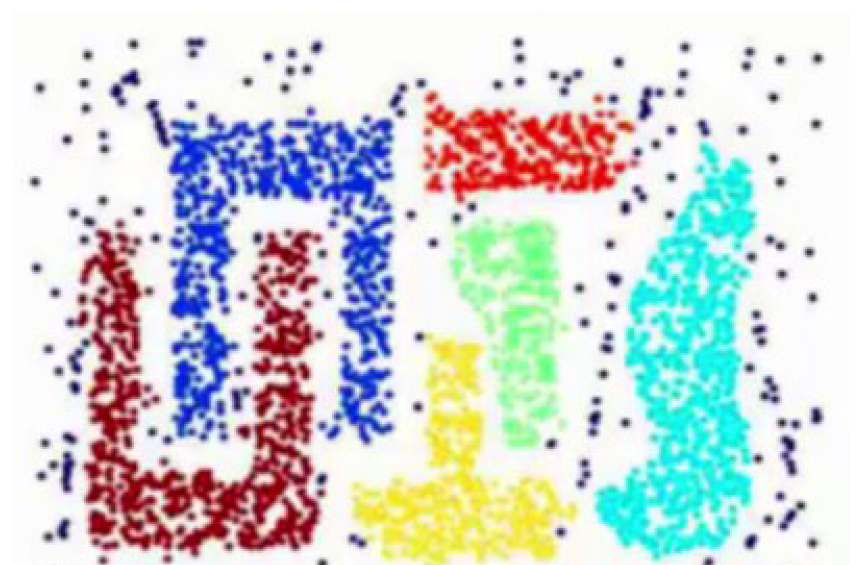
\includegraphics[width=0.55\linewidth]{ai_ml_practice/images/ch08_q05_clustering_figure.png}
\end{center}
\end{ejer}

图中簇呈非凸、弯曲形状，并含有离群噪声点，不适合用 k-means 这类偏向球形簇的算法。
宜采用\textbf{密度聚类}，典型算法为 DBSCAN。

DBSCAN 的基本思想是：若某点 $\varepsilon$ 邻域内样本数不少于 MinPts，则该点为核心点；
从核心点出发，把密度可达的点不断并入同一簇；不能并入任何簇的点视为噪声。
两个重要参数是邻域半径 $\varepsilon$ 和最小邻域样本数 MinPts。
$\varepsilon$ 太小会把一个簇切碎并产生过多噪声，太大则可能把相邻簇合并；
MinPts 太小会把噪声误认为簇，太大则会漏掉稀疏簇。

\section{第 9 章：神经网络}

\qtitle{一、TensorFlow 神经网络网页与二分类网络模型}

\begin{ejer}[TensorFlow 神经网络网页与二分类网络模型]
根据 TensorFlow 神经网络学习网页及图中二分类网络模型，解释图中 1--8 的含义，并计算该网络的参数数量。
\begin{center}
    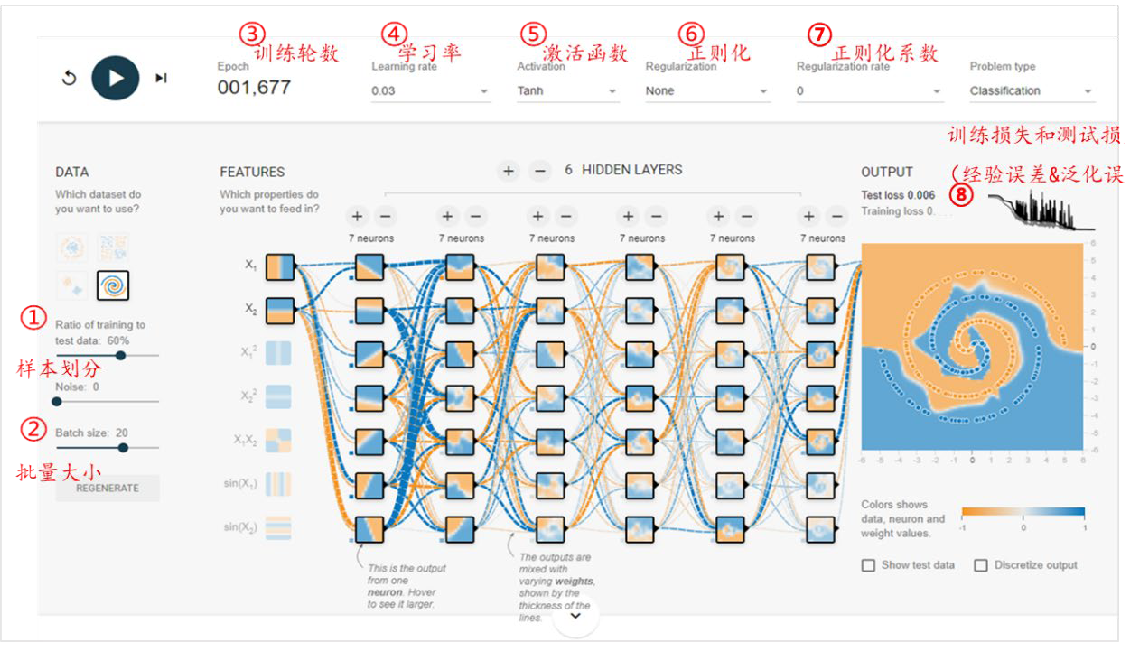
\includegraphics[width=0.78\linewidth]{ai_ml_practice/images/ch09_q01_tensorflow_network.png}
\end{center}
\end{ejer}

\begin{enumerate}[label=（\arabic*）]
    \item 图中 1--8 的含义如下。
    \begin{center}
    \begin{tabular}{cl}
    \toprule
    编号 & 含义\\
    \midrule
    $1$ & 训练集与测试集划分比例\\
    $2$ & 批量大小，即一次参数更新使用的样本数\\
    $3$ & 训练轮数 Epoch\\
    $4$ & 学习率\\
    $5$ & 激活函数\\
    $6$ & 正则化方式\\
    $7$ & 正则化系数\\
    $8$ & 训练损失与测试损失，用于观察经验误差和泛化误差\\
    \bottomrule
    \end{tabular}
    \end{center}

    \item 图中实际选用 2 个输入特征，6 个隐藏层，每个隐藏层 7 个神经元，输出层为 1 个二分类输出。
    参数量为
    \[
        (2\times7+7)+5(7\times7+7)+(7\times1+1)
        =21+280+8=309.
    \]
    因此该网络共有 $309$ 个可训练参数。
\end{enumerate}

\qtitle{二、名词解释}

\begin{ejer}[名词解释]
解释以下概念：早停法（Early stopping）、暂退法（Dropout）、梯度弥散。
\end{ejer}

\begin{description}[leftmargin=6em,style=nextline]
    \item[早停法]
    训练过程中监控验证集性能，当验证误差不再下降或开始上升时停止训练，以避免过拟合。

    \item[暂退法]
    Dropout，在训练时以一定概率随机将部分神经元输出置零，使网络不能过度依赖某些局部特征，
    相当于一种正则化方法。

    \item[梯度弥散]
    深层网络反向传播时，梯度在多层链式相乘后逐渐变得很小，导致靠近输入层的参数更新缓慢甚至难以训练。
\end{description}

\qtitle{五、BP 神经网络一次迭代}

\begin{ejer}[BP 神经网络一次迭代]
针对图中神经网络，激活函数为 $\tanh$，损失函数为带 $1/2$ 系数的平方误差，
学习率 $\eta=0.5$。计算 $h_1,h_2,o_1,o_2$ 的误差信号，并更新 $w_4,w_8,w_{01}$。
\begin{center}
    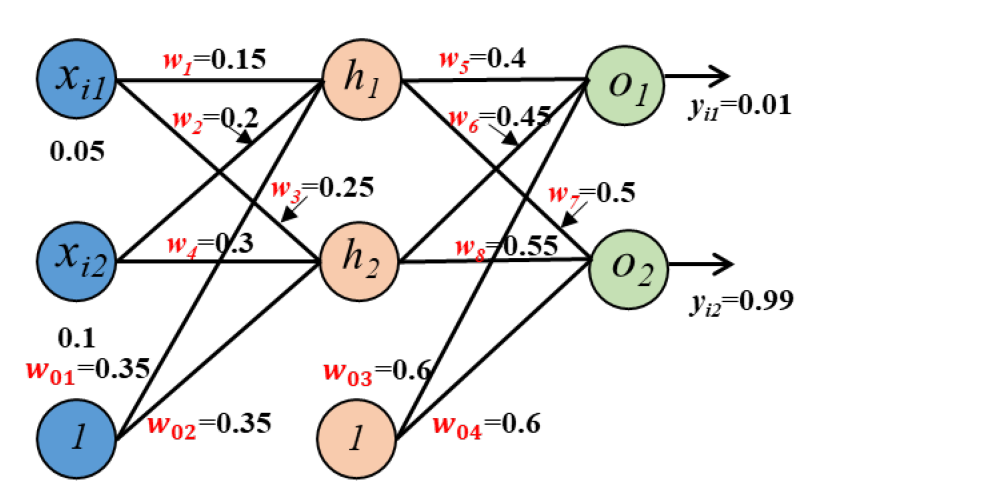
\includegraphics[width=0.68\linewidth]{ai_ml_practice/images/ch09_q05_bp_network.png}
\end{center}
\end{ejer}

采用图中权重连接关系：
$w_1:x_1\to h_1$，$w_2:x_1\to h_2$，$w_3:x_2\to h_1$，$w_4:x_2\to h_2$；
$w_5:h_1\to o_1$，$w_6:h_1\to o_2$，$w_7:h_2\to o_1$，$w_8:h_2\to o_2$。
激活函数为 $\tanh z$，其导数为 $1-\tanh^2z$。前向传播得
\[
    net_{h_1}=0.3825,\quad h_1=0.364877,
\]
\[
    net_{h_2}=0.3900,\quad h_2=0.371360,
\]
\[
    net_{o_1}=0.931631,\quad o_1=0.731353,
\]
\[
    net_{o_2}=0.968443,\quad o_2=0.748019.
\]
以下采用误差信号
\[
    \delta_j=-\frac{\partial E}{\partial net_j}.
\]
输出层
\[
    \delta_{o_1}=(y_1-o_1)(1-o_1^2)=-0.335518,
\]
\[
    \delta_{o_2}=(y_2-o_2)(1-o_2^2)=0.106585.
\]
隐藏层
\[
    \delta_{h_1}=(1-h_1^2)(w_5\delta_{o_1}+w_6\delta_{o_2})=-0.074762,
\]
\[
    \delta_{h_2}=(1-h_2^2)(w_7\delta_{o_1}+w_8\delta_{o_2})=-0.094086.
\]
用 $w\leftarrow w+\eta\delta\cdot input$，$\eta=0.5$，得到
\[
    w_4'=0.3+0.5(-0.094086)(0.1)=0.295296,
\]
\[
    w_8'=0.55+0.5(0.106585)(0.371360)=0.569791,
\]
\[
    w_{01}'=0.35+0.5(-0.074762)=0.312619.
\]

\qtitle{六、BGD 的 BP 神经网络训练步骤}

\begin{ejer}[BGD 的 BP 神经网络训练步骤]
简述采用批量梯度下降（BGD）的 BP 神经网络训练步骤。
\end{ejer}

批量梯度下降的 BP 训练步骤如下：初始化网络权重和偏置；对整个训练集做前向传播，计算每个样本输出和总损失；
从输出层开始反向传播，计算各层误差信号；对全体训练样本的梯度求和或求平均；
用平均梯度一次性更新所有参数；在验证集上检查性能并判断是否达到停止条件；重复以上过程直到收敛或达到最大轮数。

\qtitle{七、Softmax 与交叉熵}

\begin{ejer}[Softmax 与交叉熵]
10 分类网络输出层采用 Softmax。真实标记第 6 维为 $1$，网络输出为
\[
(0.2,0.1,0,0,0,0.4,0,0.15,0.15,0)^T.
\]
计算交叉熵损失；若前一隐层神经元输出 $h=0.128$，连接权重为
\[
W=(0.1,-0.1,0.2,-0.2,0.3,-0.3,0.4,-0.4,0.5,-0.5)^T,
\]
学习率 $\eta=0.1$，更新该权重向量。
\end{ejer}

\begin{enumerate}[label=（\arabic*）]
    \item 真实类别是第 6 类，预测概率为 $0.4$，因此交叉熵损失为
    \[
        L=-\log 0.4=0.9163.
    \]

    \item Softmax 与交叉熵组合时，输出层第 $j$ 个权重的梯度为
    \[
        \frac{\partial L}{\partial W_j}=h(\hat y_j-y_j).
    \]
    这里 $h=0.128$、$\eta=0.1$，所以
    \[
        W'=W-0.1\times0.128(\hat y-y).
    \]
    代入得
    \[
    W'=
    \begin{pmatrix}
    0.09744\\
    -0.10128\\
    0.20000\\
    -0.20000\\
    0.30000\\
    -0.29232\\
    0.40000\\
    -0.40192\\
    0.49808\\
    -0.50000
    \end{pmatrix}.
    \]
\end{enumerate}

\section{第 10 章：深度学习}

\qtitle{九、卷积层参数量}

\begin{ejer}[卷积层参数量]
一个卷积神经网络输入为 $32\times32\times3$ 图像，第一个隐藏层卷积核大小为
$5\times5$，共有 10 个卷积核。计算该层参数总量，含偏置参数。
\end{ejer}

输入通道数为 $3$，每个卷积核大小为 $5\times5$，因此一个卷积核含
\[
    5\times5\times3=75
\]
个权重。每个卷积核再配一个偏置参数，共 $76$ 个参数。
该层有 $10$ 个卷积核，所以总参数量为
\[
    10\times(75+1)=760.
\]

\end{document}
